\documentclass{article}

\usepackage{tikz}
\usepackage{amsthm,amsmath,amssymb}
\usepackage{csquotes}
\usetikzlibrary{automata}
\usetikzlibrary{graphs}

\theoremstyle{definition}
\newtheorem{defn}{Definition}

\begin{document}

\section{Formal Verification of Flexibility in Swarm Robotics}

Microscopic v.s. macroscopic
approach to model checking
swarm robotics.

"The first approach consists of building a model by first creating a corresponding
finite state machine for each robot behavior and then by taking the composition of
all those finite state machines. The second approach consists of building a single
finite state machine containing a state for each different sub-behavior of the robots.
Each state is associated with a counter that keep track of the number of robot
currently in that state."

\section{Transition System Representing a Battle}

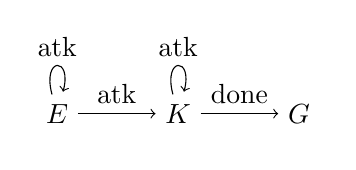
\begin{tikzpicture}
    \matrix[row sep=2cm, column sep=1cm]{
        \node (E) {$E$} ; &
        \node (K) {$K$} ; &
        \node (G) {$G$} ; \\
    } ;

    \graph[use existing nodes] {
         E -> [edge label={atk},loop above]
         E ->[edge label={atk}]
         K ->[edge label={atk},loop above]
         K ->[edge label={done}] G ;
    } ;
\end{tikzpicture}

At the beginning of each battle, some number
of robots are assigned to fit enemy $ i $,
which is represented in state E. In state E,
the action "attack" can be taken. This action
will probabilistically result in the defeat
of the enemy, or require additional attacks.

The probability of neutralizing an enemy
is given in the next section.

If the attack succeeds, then the battle transitions
to the "complete" phase (state K), upon which
all robots get redistributed to the other
battles that are being fought (concurrently)!
Furthermore, we must set the base level of the
freshly defeated enemy as 0.

Because we create a product transition system
in which the action "attack" is a handshake action,
we include a dummy "attack" action in state K
that goes to itself, in order to allow other
battles to continue.

Upon the completion of all battles, there is a
"done" action that can be taken (also a handshake action)
that allows all battles to reach
the "goal" state simultaneously, thus
concluding the engagement.

Future extensions: Attacks could probabilistically result
in casualties.

\section{The Role of Probability}

As discussed, the event of defeating some enemy
occurs probabilistically. We have heterogeneous
enemies, which we model by assigning them
"levels". Conceptually, enemies with higher
levels are more difficult to defeat than other
enemies (i.e. the probability of defeating an
enemy in an attack is lower).

However, conceptually it also makes sense that
a higher number of robots attacking the same
enemy would make it more likely that an enemy
is defeated in a round of combat.

Hence, we define the probability of \textbf{not defeating}
an enemy in a round of combat using the following
function of the level of the enemy
(the cumulative distribution function of the
exponential distribution).

$$ f(l_i) = 1 - e^{-\lambda_i l_i} $$

This is motivated by the idea of dynamically adjusting the
probability of not defeating an enemy as there
are more robots fighting it.

$ \mathcal{l}_i $ is the base level of an enemy.
Then, we say that $ \lambda_i = \frac{1}{cn_i + 1} $ is the adjustment
factor, where $ n_i $ is the number of robots
currently fighting enemy $ i $, and $ c $ is a
hyperparameter that describes robot neutralization efficiency.
1 must be added to avoid division by zero problems.

\section{Optimization}

Roughly stated, the ultimate goal is to find the optimal
portioning of robots to minimize the number of rounds of
combat in order to successively neutralize all targets.

\begin{displayquote}

    We have N robots.

    Let $ \mathcal{M} = \{m_1, m_2, \ldots, m_k \} $ be the set of all enemies.

    Further, let L be the bound in $ \mathcal{L} = \{ 1, \ldots, L \} $.

    Our goal is to find a function $ L^\mathcal{M} \to [0,1]^\mathcal{M} $
    such that the expected number of turns to neutralize all enemies
    is minimized.

\end{displayquote}

This function takes ordered tuples of enemies levels (the remaining battles),
and produces a probability distribution
over them that is used to inform the proportions by which the newly unallocated
robots are distributed among the remaining battles.

Because arbitrary functions cannot be described in PRISM, we have assumed
that the distribution of robots over the remaining battles will simply be the weighted distribution
by current adjusted level (what we previously called $ \lambda_i l_i $).

However, we would like to be able to tune the function in order
to optimize how robots are (re)distributed among battles.
For our initial experiment, we choose the function $ g(x) = x^a $,
where $ a $ is a parameter that will be tuned using
simulated annealing (by verifying desired properties repeatedly
using different values of $ a $). This function can be interchanged
with any other function in order to achieve the desired scaling amount
for redistribution.

Thus, we can now define our
function $ L^\mathcal{M} \to [0,1]^\mathcal{M} $ as follows:

$$ f(\langle l_1, \ldots, l_k \rangle) = \frac{g(\langle \lambda_1 l_1, \ldots, \lambda_k l_k \rangle)}{\sum_j^{g(\langle \lambda_j l_j \ldots \lambda_k l_k \rangle)}} i \in \{1, \ldots, M\} $$

We assume that the functions g and f operate element-wise on tuples.

We assume that all of our robots are homogeneous.
However, our enemies are assumed to be heterogeneous
(as defined using our level system).

\end{document}
